\subsection{Direct Detection}
\label{sec_ddphen}
In this section the phenomenological aspects of DM itself are focussed.
We start with direct detection (DD) or nucleon ($N$) scattering where a DM particle scatters off a parton (quark or gluon) of a nucleon. 
\\ \\ \textit{Effective Lagrangian}\\
The process arises
due to a spin independent (SI) or spin dependent (SD) interaction \eqref{eq_th.sigma.dd} which are described by an effective Lagrangian \cite{1104.0228}
\begin{align}
 \mathcal{L}^\text{eff} = \sum\limits_{q,Q} \mathcal{L}^\text{eff}_{q,Q} + \mathcal{L}^\text{eff}_g.
\end{align}
We use $q$ for the light quarks $u$, $d$, $s$ and $Q$ for heavier $c$, $b$, $t$ and $g$ for gluons. \eqref{eq_fierzSPtoVA} shows that this chiral model
only provides effective interactions with quarks as $\bar \chi\gamma^\mu\chi \bar q\gamma_\mu q$ and $\bar \chi\gamma^\mu\gamma_5 \bar q\gamma_\mu \gamma_5 q$
as six dimensional operators. The former vanishes for Majorana DM. The latter is SD 
and the resulting cross section can be evaluated with the expressions given in \cite{1104.0228} for the leading processes to be of
order $\mathcal{O}(10^{-44})$ cm$^2$. But the upper limits obtained by IceCube \cite{1212.4097} yield $\mathcal{O}(10^{-40})$ cm$^2$ for 
a 100 GeV DM particle.
Therefore, we can neglect them. A possibly occurring scalar operator $f_q m_q\bar \chi \chi \bar q q$ also vanishes for tree level processes in our chiral model
but is enabled at loop level. Therefore, the first contributing
SI operators coming from quark interactions are eight dimensional, namely those depending on twist-2 operators. They are the traceless parts of the
quark energy momentum tensor and arise from the matrix element of a quark current product expressed in local operators \cite{MDSchwartz}. 
% The twist of an operator is definded as the difference between its mass dimension and its spin. 
\\ \noindent Since our DM particle shall be an 
$SU(3)_C$-singlet, it does not couple directly to gluons $g$ but scalar-like at one-loop level through the heavy quarks. There is also a twist-2 
operator for the gluon but its coefficient will be suppressed by $\alpha_s$ so we will not consider it further. For the $SU(2)_L$ singlet
DM particle, which does not interact with the $W$ bosons, the leading SI Lagrangian is
%For both DM $SU(2)_L$-representations, the singlet and the triplet, the leading SI operators are
\begin{align}
 \mathcal{L}^\text{eff} =&\, \frac{g_q^{(1)}}{m_\chi} \bar \chi\ti \partial_\mu \gamma_\nu\chi O_q^{\mu\nu} + \frac{g_q^{(2)}}{m^2_\chi} \bar \chi(\ti \partial_\mu) (\ti\partial_\nu)\chi O_q^{\mu\nu} \\
 \nonumber
 &+ f_G \bar \chi \chi G^a_{\mu\nu} G^{a\mu\nu}.
\end{align}
The twist-2 operator for the quark is
\begin{align}
 O_q^{\mu\nu} = \frac12 \bar q \ti \left(D^\mu \gamma^\nu + D^\nu \gamma^\mu - \frac12 g^{\mu\nu} \slashed{D}\right) q
\end{align}
with $D_\mu$ as the covariant derivative for $SU(3)_C$. The three coefficients of mass dimension $-3$ ($g_q^{(1)}$, $g_q^{(2)}$, $f_G$) enter 
the form factor $f_N$ in \eqref{eq_th.sigma.dd} as
\begin{align}
 \frac{f_N}{m_N} = \sum\limits_{q,c,b} \frac34 \left(q(2)+\bar q(2)\right) \left(g_q^{(1)} + g_q^{(2)}\right) - \frac{8\pi}{9\alpha_s}f_{TG}f_G
 \label{eq_ddformfactorA}
\end{align}
where the matrix elements of the effective operators are expressed with the nucleon mass $m_N$ as \cite{1007.2601}
\begin{subequations}
\begin{align}
 \langle N(p)| O_q^{\mu\nu} | N(p)\rangle =& \frac{1}{m_N}\left(p^\mu p^\nu - \frac14 m_N^2 g^{\mu\nu}\right) \left(q(2) + \bar q(2)\right),\\
 f_{TG} :=& 1- \sum\limits_q f_{Tq},\\
 f_{Tq} :=& \langle N|m_n \bar qq |N\rangle /m_N.
\end{align}
\end{subequations}
The quantities $q(2)$ and $\bar q(2)$ are the second moments \cite{0811.1779} of the parton distribution function (PDF) of quark $q(x)$ or antiquark 
$\bar q(x)$, respectively, in the nucleon ($q(2)+\bar q(2) = \int_0^1 \dx x\, x^2 \left[q(x) + \bar q(x)\right]$). The values used for the numerical
calculation are listed in table \ref{tab_parton}.
\begin{table}[b]
 \begin{tabular}{c|ccccc}
   & $u$ & $d$ & $s$ & $c$ &$b$ \\
   \hline
  $q(2)$ & 0.22 & 0.11 & 0.026 & 0.019 & 0.012\\
  $\bar q(2)$ & 0.034 & 0.036 & 0.026 & 0.019 & 0.012\\
  $f_{Tq}$ & 0.020& 0.026 &\hspace{0.47cm}  0.134\cite{1209.3641}\\
 \end{tabular}
\caption{Second moments $q(2)$, $\bar q(2)$ of the quark PDFs evaluated at $\mu=m_Z$ and taken from \cite{0201195} and scalar matrix elements $f_{Tq}$ of 
the light quarks for the 
proton each. For the neutron $u(2)$ and $d(2)$ just swap and $f_{Tu}$ and $f_{Td}$ differ slightly \cite{9506380}. All other quantities are the same. }
\label{tab_parton}
\end{table}
\noindent The evaluation of $f_G$ is factorised in a short distance and a long distance 
contribution. The former (latter) represents a scale of heavy (light) particles as the coloured scalar mediator (quarks). 
While the full loop process has to be calculated for the short distance (see fig. \ref{pic_ddsinglet}c), the long distance term can be thought of
as a triangle diagram (see fig. \ref{pic_ddsinglet}b) where $\Phi_q$ integrated 
out i.e. there arises a four fermion operator $f_Q m_Q \bar \chi \chi\bar Q Q$. The long distance gluonic form factor is expressed by $f_Q$ 
which are multiplied by a constant 
$c_Q = 1+11\alpha_s(m_Q)/4\pi$, ($c_c=1.32$, $c_b = 1.19$, $c_t = 1$)
resulting from large QCD corrections \cite{Djouadi}.
Due to their masses being smaller than $\Lambda_\text{QCD} = \mathcal{O}$(100 MeV), light quarks $q$ have a vanishing contribution to the long
distance term. Thus, we do not have to take them into account. The operator coefficients \eqref{eq_ddformfactorA} are determined for the 
singlet case.
\\ \\ \textit{Singlet Dark Matter}\\
\begin{figure}[t]
 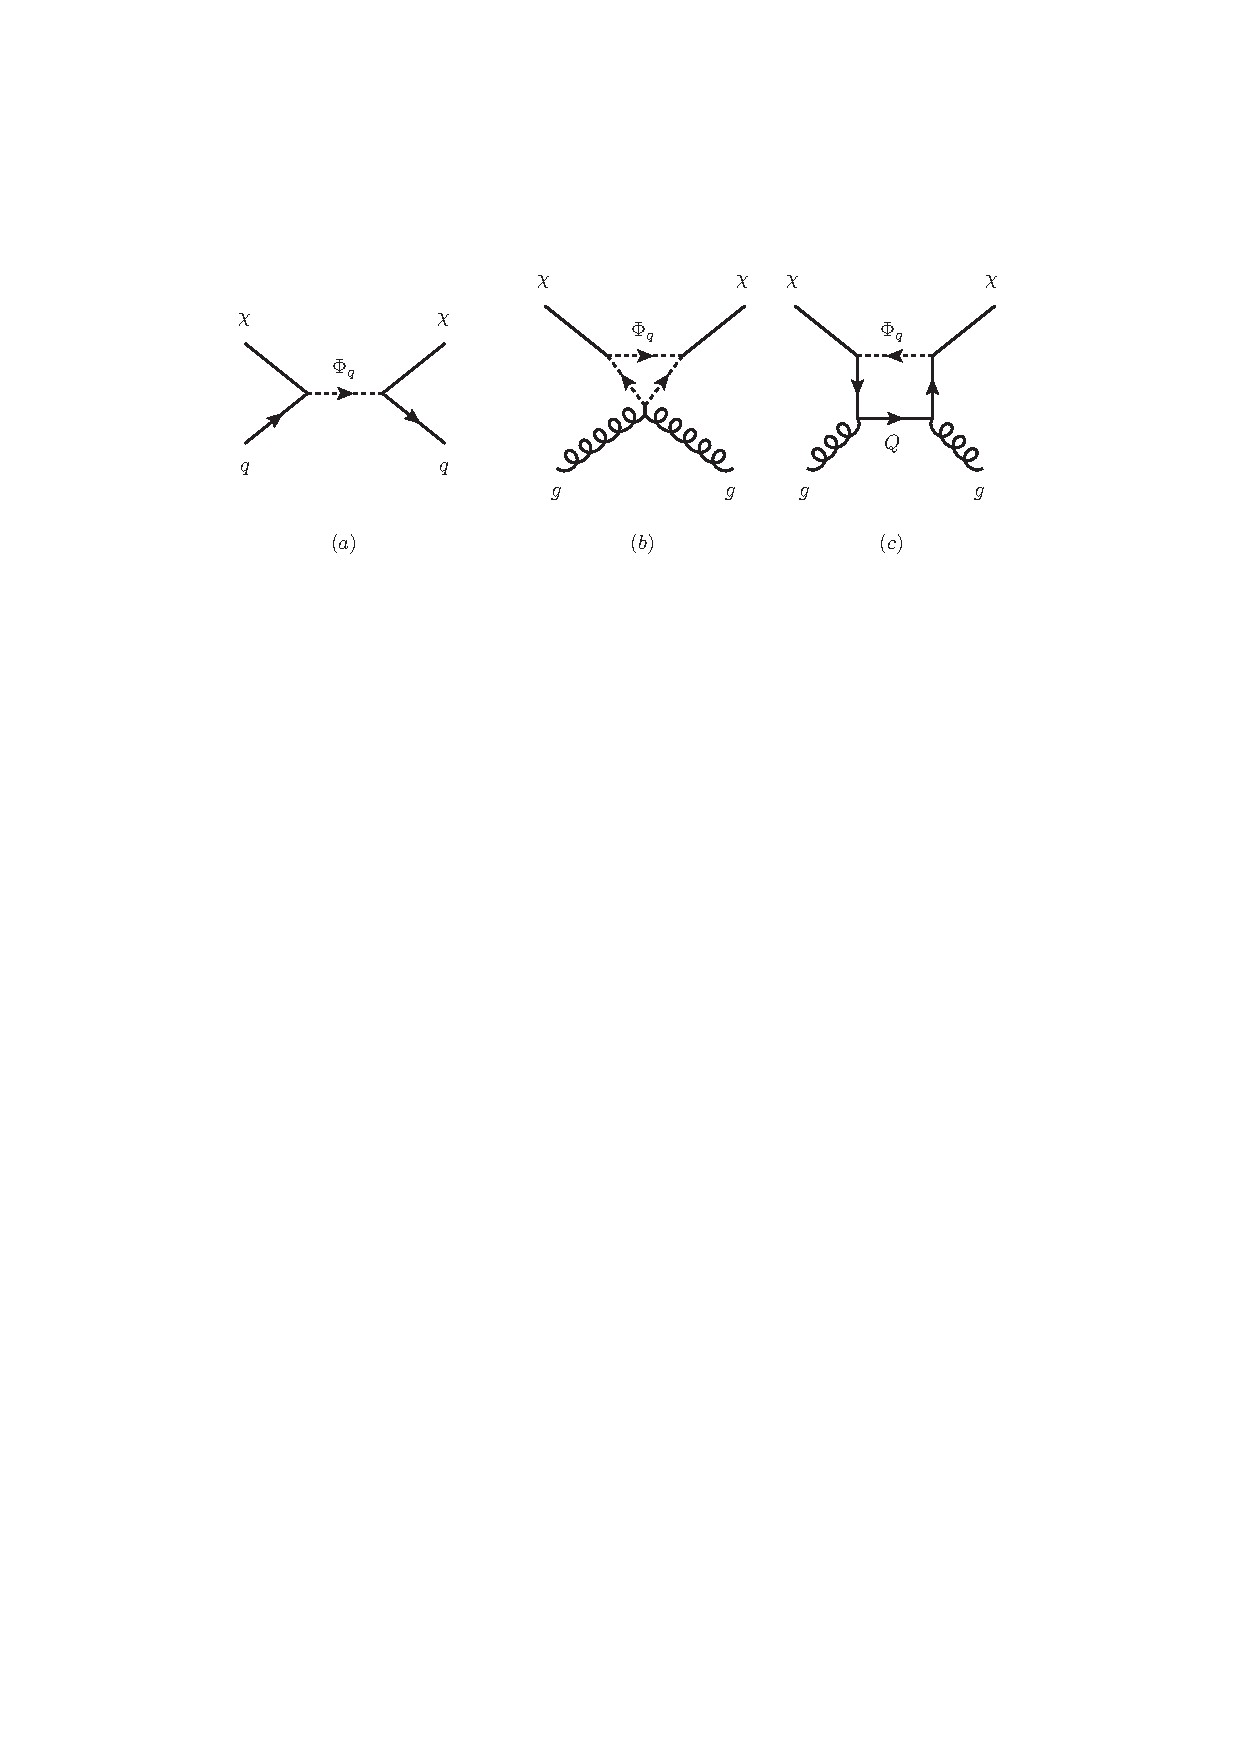
\includegraphics[width=1\textwidth]{../pics/ddsinglet.pdf}
 \caption{DM scatters off quarks at tree level and off gluons at one loop order.}
 \label{pic_ddsinglet}
\end{figure}
\noindent The $\chi$-$q$ interaction is visualised in figure \ref{pic_ddsinglet}a and is expressed by this s-channel process. After integrating out 
the scalar and in the massless quark limit the coefficients are
\begin{align}
 g_q^{(1)} = \frac{|g_q|^2 }{4} \frac{m_\chi}{\left(m_\chi^2 - M_{\Phi_q}^2\right)^2},\hspace{3cm} g_q^{(2)} = 0.
\end{align}
We assume the scalar to be much heavier than the fermion which is why possible divergences due to mass degeneracy of DM and messenger have not
to be considered. 
The effective gluonic coupling in the 
singlet case is derived from the loop processes (see fig. \ref{pic_ddsinglet}b, c) 
% \begin{figure}[t]
%  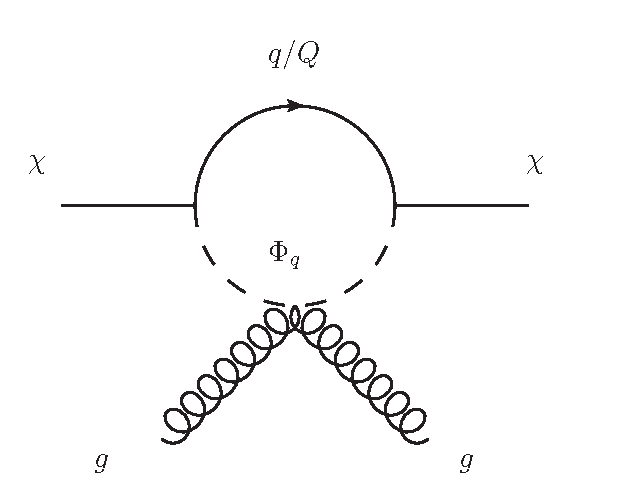
\includegraphics[width=0.5\textwidth]{../pics/phigluon.eps}
%  \caption{One loop diagrams contributing to the effective gluonic coupling.}
%  \label{pic_ddGluonA}
% \end{figure}
where we use the Fock-Schwinger gauge for the gluon
field $x^\mu G^a_\mu = 0$. The short distance (S) and long distance (L) terms are
\begin{align}
 f_G^\text{S}|_q = \frac{\alpha_s}{32\pi} m_\chi f^s,\hspace{3cm} f_G^\text{L}|_q = \frac{\alpha_s}{32\pi} m_\chi f^l
 \label{eq_ldsdLoop}
\end{align}
The loop functions $f$ (see \eqref{eq_singletloop}) are used at zero quark mass and the scalar mass being much larger than the DM mass.
In total, the scalar $\chi$-$g$ interaction coefficient reads
\begin{align}
 f_G = -\frac{\alpha_s}{96\pi} \frac{m_\chi}{M_{\Phi_q}^4} \sum\limits_{\text{all}} |g^q|^2
\end{align}
and the full form factor \eqref{eq_ddformfactorA} can be written in these limits as
\begin{align}
 \frac{f_N}{m_N} = \frac{m_\chi}{M_{\Phi_q}^4} \sum\limits_{q,Q} \left|g^q\right|^2 \left[\frac{f_{TG}}{108} + \frac{3}{12}\left(q(2) + \bar q(2)\right)\right].
 \label{eq_siformsinglet}
\end{align}
With their high Yukawa couplings, the bottom and top quark dominate the form factor. Inserting \eqref{eq_siformsinglet} into \eqref{eq_th.sigma.dd}
yields for a 100 GeV DM fermion and a 1 TeV messenger, the SI $\chi$-$N$ cross section computes to $\mathcal{O}(10^{-49}$ cm$^2$). This is far below
current bounds. Hence, testing the singlet case by direct detection is currently impossible.
\\ \\ \textit{Triplet Dark Matter}\\
\begin{figure}[t]
 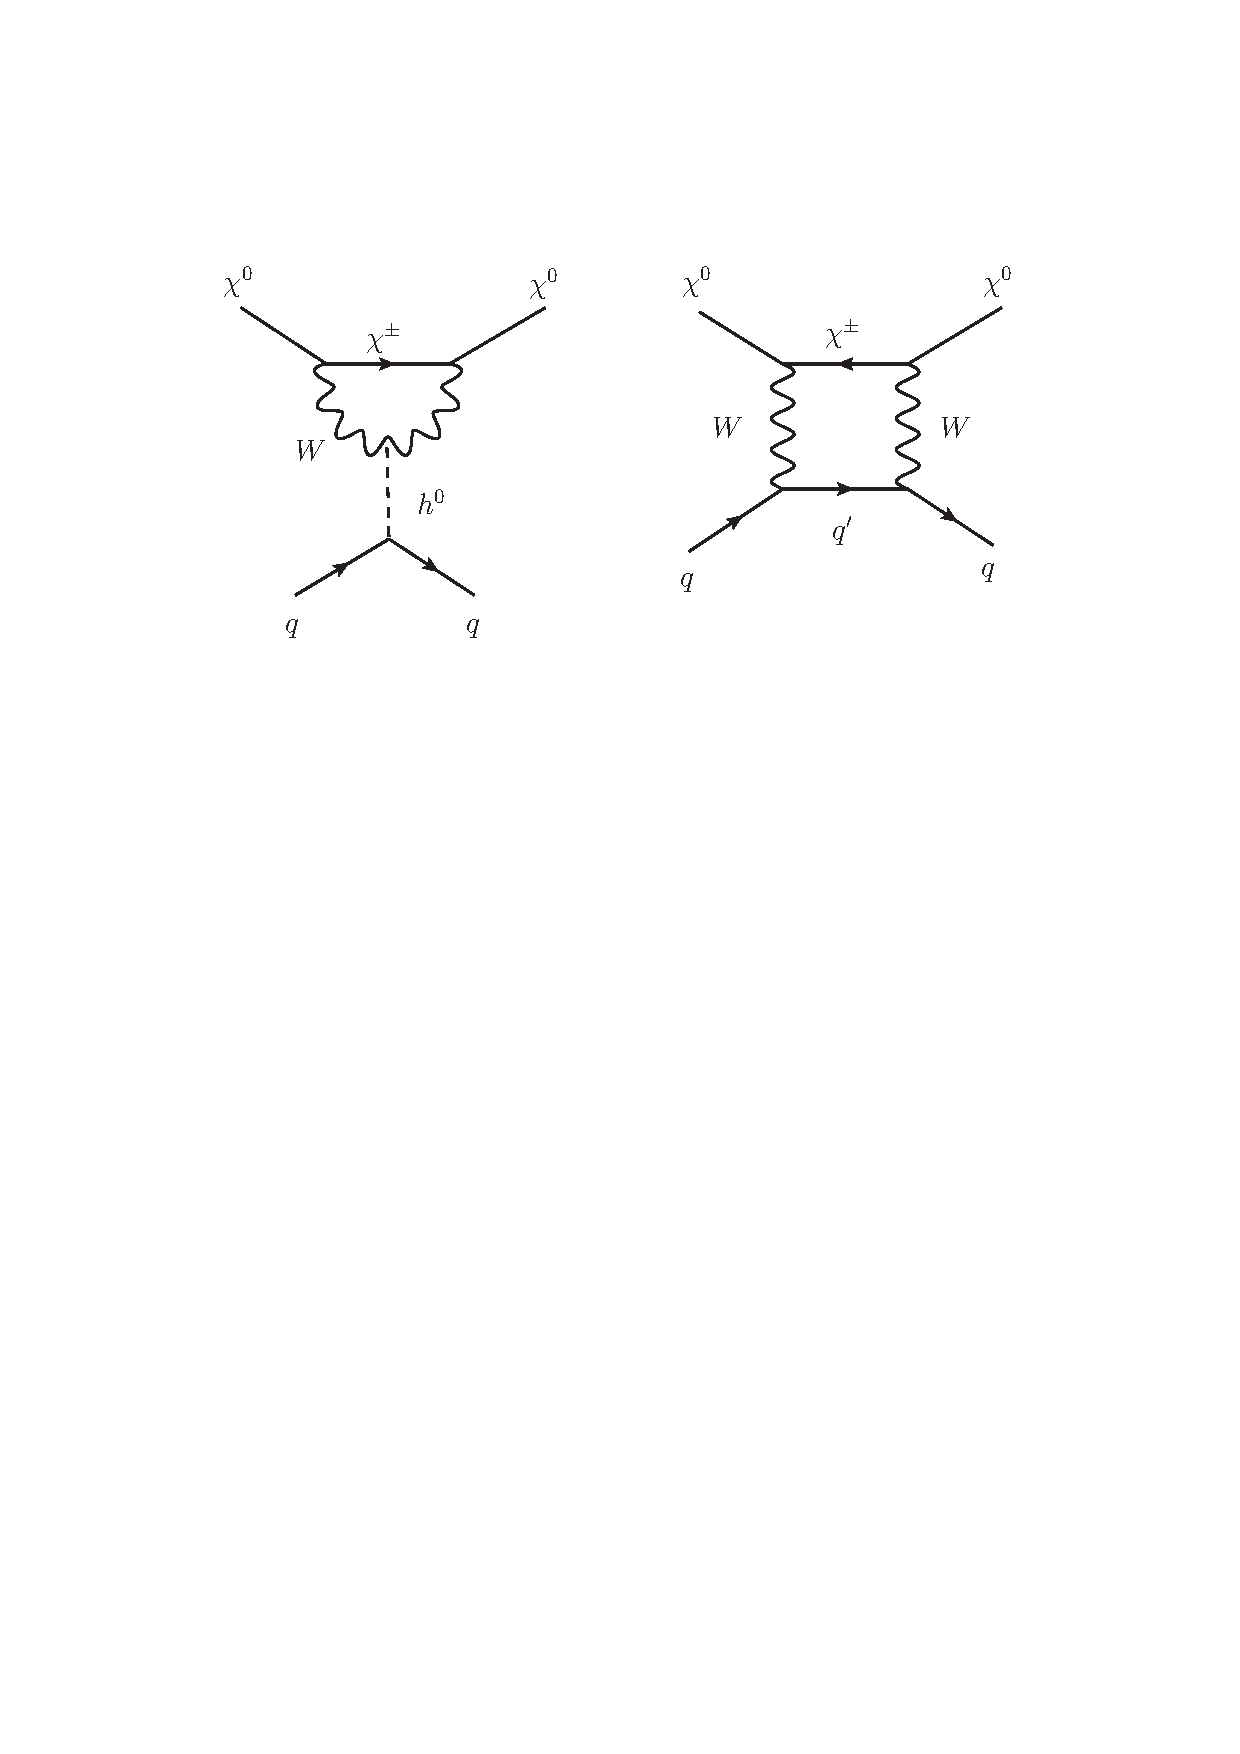
\includegraphics[width=0.7\textwidth]{../pics/wloops.pdf}
 \caption{One loop processes for the effective $\chi^0-N$ coupling. Penguins with a photon or a $Z$-boson turn out to vanish(\cite{1104.0228}).}
 \label{pic_wloop}
\end{figure}
\noindent The main difference between the $SU(2)_L$ singlet and the triplet is the interaction with the weak boson $W$. While the singlet does not couple to
it directly, the $W$ couples to two particle states within the triplet whose electric charges differ by one. To remind, in neither case the 
DM particle carries hypercharge, so that the respective neutral component does not couple to the $Z$ boson. The interaction Lagrangian with the $W$ 
boson is 
\begin{align}
 \mathcal{L} = \frac{g_2}{\sqrt{2}} \left[\bar \chi^0 \gamma^\mu \chi^- W^+_\mu + \bar \chi^0 \gamma^\mu \chi^+W^-_\mu\right] +\, \text{h.c.}
\end{align}
Since the cross section in the singlet case was suppressed by the large scalar mass we can take advantage of the possible 
processes for direct detection which do not involve the scalar \cite{1004.4090}. In fact, the form factor is dominated by one loop processes with a 
$W$ for an interaction with quarks (see fig. \ref{pic_wloop}) and two loop processes for gluonic scattering (see fig. \ref{pic_2loopgluon}).
\begin{figure}[t]
 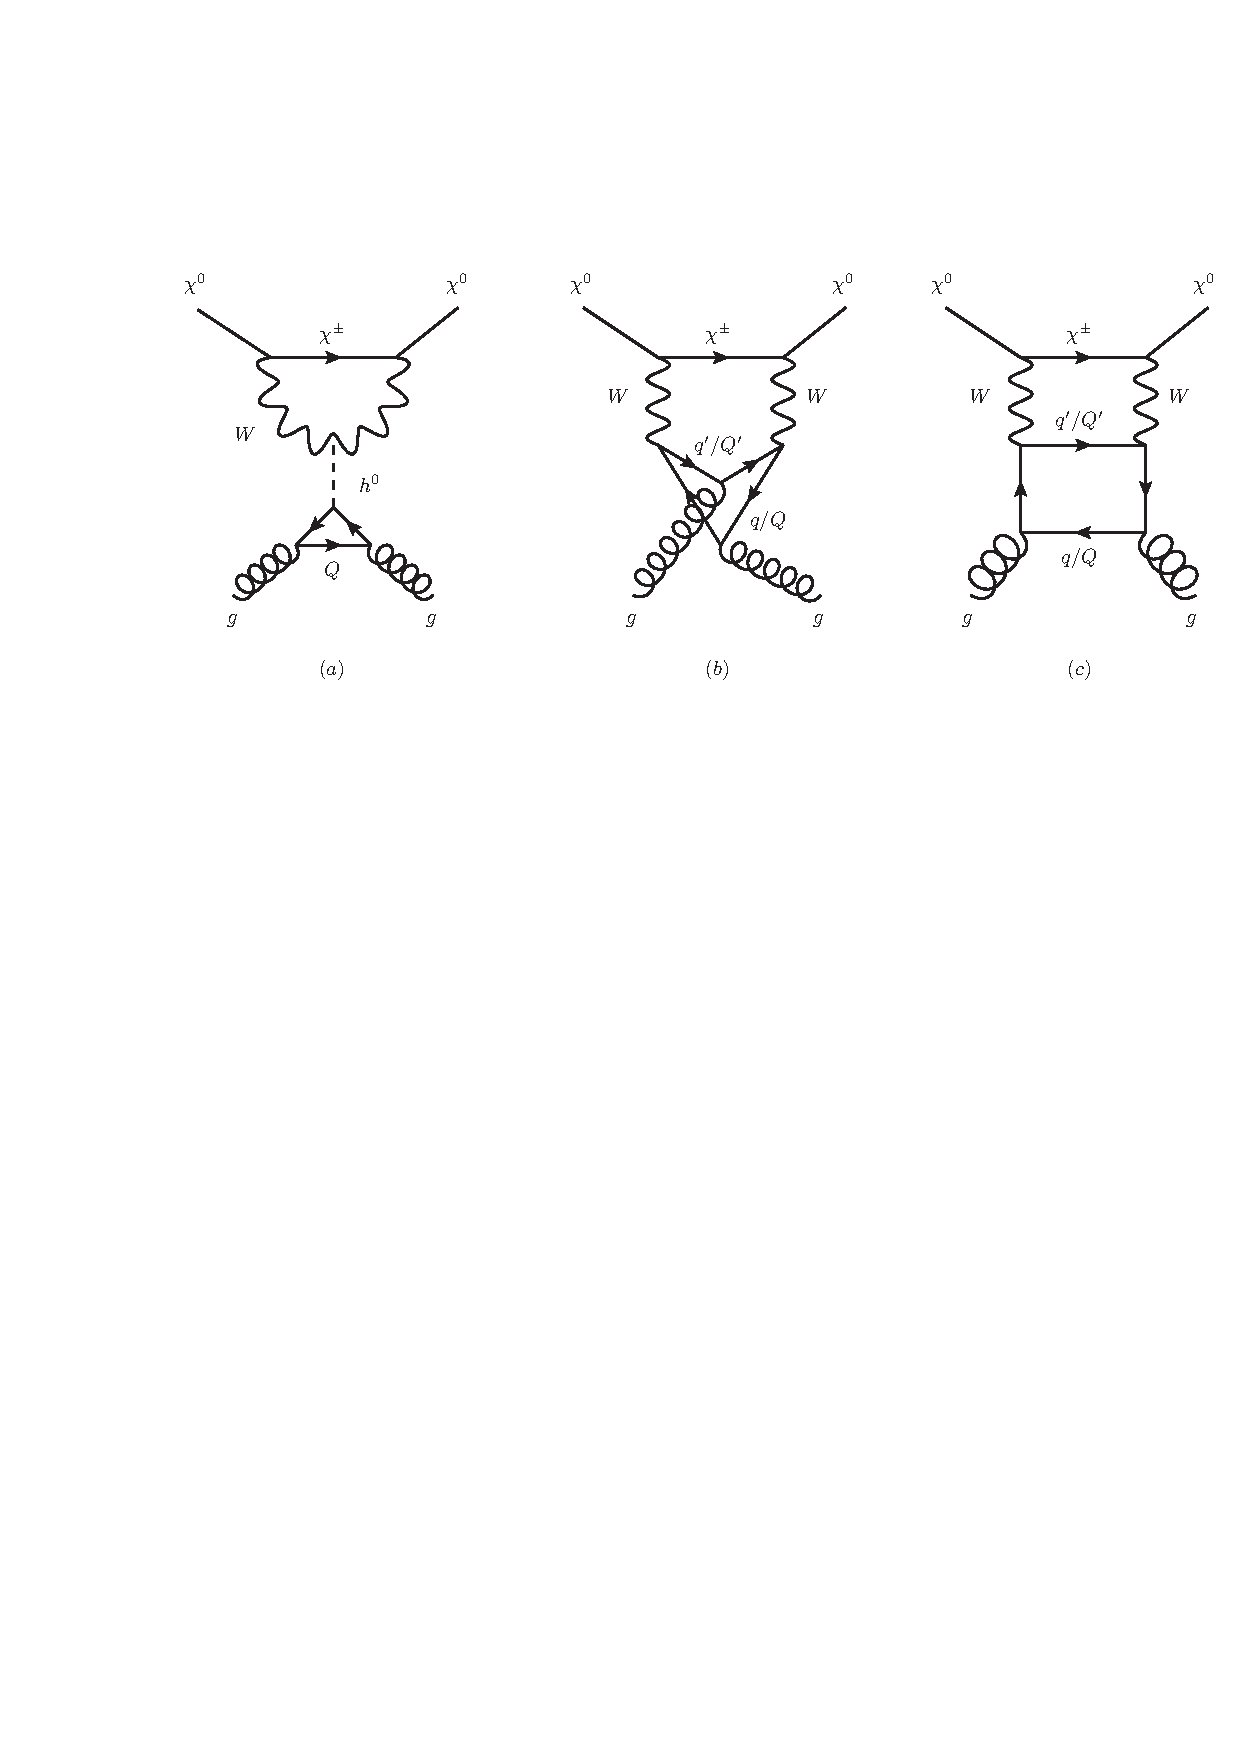
\includegraphics[width=1\textwidth]{../pics/gluon2loopB.pdf}
 \caption{Two loop diagrams contributing to the effective gluonic coupling.}
 \label{pic_2loopgluon}
\end{figure}
For the effective $\chi^0$-$q$-coupling follows
\begin{align}
 f_q =& \frac{\alpha_2^2}{4m_W m_{h}^2} g_H(w),\\
 g^{(1)}_q =& \frac{\alpha_2^2}{m_W^3}g_{T1}(w),\\
 g^{(2)}_q =&\frac{\alpha_2^2}{m_W^3}g_{T2}(w), 
\end{align}
where $f_q$ gets its contributions from $h^0$ exchange and the $W$-box leads to $g^{(i)}_q$. The $W$-mass and the Higgs-mass are denoted by$m_W$ and 
$m_h$, respectively. The function argument is $w=\sfrac{m_W^2}{m_\chi^2}$ \\
\noindent Concerning the gluonic coupling, there are three dominating two loop processes, one via Higgs exchange (fig. \ref{pic_2loopgluon}a) and two
via $W$-boxes (fig. \ref{pic_2loopgluon}b, c). The first one is evaluated by comparing it to the effective quark coupling from figure \ref{pic_wloop}a
by exchanging the light scattered quarks with heavy loop quarks which hence contributes to the long distance interaction. 
The calculation of the other two diagrams is quite extensive since the loops have to be calculated explicitly with the additional treatment of the vacuum 
polarisation tensor of the $W$ \cite{1007.2601}. In the end we have for the effective $\chi^0$-$g$ coupling reads
\begin{align}
 f_G = \frac{\alpha_s\alpha_2^2}{4\pi m_W}\left(-\sum\limits_Q c_Q \frac{1}{3m_{h^0}^2} g_H(w) + \frac{1}{m_W^2} g_{W}(w,t) \right)
\end{align}
with $t=\sfrac{m_t^2}{m_\chi^2}$ ($m_t$ is the top mass).
With the additional scalar $\chi^0$-$q$ coupling giving a contribution to the form factor as $\sum_qf_{Tq}f_q$, the result is
\begin{align}
 \frac{f_N}{m_N} &= \frac{\alpha_2^2}{m_W^3}\left(\sum\limits_{q,c,b} \frac34 \left(q(2)+\bar q(2)\right) \left(g_{T1}(w) + g_{T2}(w)\right) + \frac29g_W(w,t)\right) \\
 \nonumber
 &+ \frac{\alpha_2^2}{m_W m_h^2}g_H(w) \left(\frac14 \sum\limits_q f_{Tq} - \frac{2}{27}f_{TG}\sum\limits_Q c_Q \right).
\end{align}
As stated in the beginning of this section, the cross section only depends
on $m_\chi$. The mass difference of the charged triplet components to the neutral one is assumed to be negligible compared to the mass scale itself,
so they do not enter explicitly. 

% \begin{align}
%  \sigma_\text{SI} = \frac{4}{\pi}\mu_N^2 \left| f_N \right| ^2 \approx 4.57\cdot 10^{-18} \mu_N^2 \cdot \left(0.51 \left(g_{T1}+g_{T2}\right) + \frac29 g_W - 0.02 g_H\right)
%  \label{eq_sigmaDDB}
% \end{align}
% with the masses in GeV. Unlike \eqref{eq_sigmaDDA} the cross section for the triplet case only depends on the DM mass which makes it generally very
% interesting in constraining such models. 











